\documentclass[aspectratio=169]{beamer}
\beamertemplatenavigationsymbolsempty

\mode<presentation>
{
        \usetheme{Singapore}
        % \useoutertheme{}
	\setbeamercovered{transparent}
	\setbeamertemplate{footline}[frame number]
}

% \usepackage{flashmovie}
\usepackage[utf8]{inputenc}
\usepackage[T1]{fontenc}
%\usepackage[ngerman]{babel}
\usepackage[english]{babel}
\usepackage{amsmath}
\usepackage[absolute,overlay]{textpos}
\usepackage{svg}

\usebackgroundtemplate{%
\begin{tikzpicture}[remember picture,overlay]
\node[anchor=south west] at (current page.south west) {\includegraphics[height=0.4cm]{by.eps}};
\end{tikzpicture}}

\author[]{Anton Kuzmin}
\institute[]{}
\date[]{@DATE@}

\usepackage{tikz}

\title[GMM-7550 Module]{GMM-7550 -- Cologne Chip GateMate FPGA Module}
\subtitle{}

\setbeamerfont{table font}{size=\tiny}

\begin{document}

\begin{frame}
  \titlepage
\end{frame}

\section{Introduction}

\begin{frame}
  \frametitle{Who am I\dots}
  \begin{itemize}
  \item not a software developer (any more)\\
    \dots but still write code sometimes
  \item developing embedded and real-time systems for almost 30 years
  \item CAMAC, VME, CompactPCI, AdvancedTCA, SoMs
  \item FPGA and SoC-FPGA (Altera/Intel, Microsemi/Microchip)
  \item VHDL
  \end{itemize}
  \vskip.5cm

%  My usual problem with the software is how to make it run on a
%  hardware which is known not to be working yet and how to bring-up
%  and test this hardware. With a soft-core CPU it is getting even
%  worse.

\end{frame}


%\frame{\tableofcontents[subsectionstyle=show]}
\frame{\tableofcontents}

\section{Motivation and Current State}

\begin{frame}
  \frametitle{Why GateMate FPGA}

  \begin{itemize}
    \item a new kid on the block
    \item FOSS commitment (Yosys for synthesis right now, \texttt{nextpnr}
    announced)
    \item semi-documented (and semi-open) bitstream format
    \item possibility to change configuration at run-time from inside
  \end{itemize}

  \begin{center}
    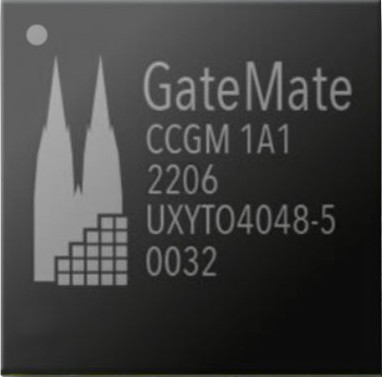
\includegraphics[height=3cm]{CCGM1A1_front.jpg}
  \end{center}

\end{frame}

\begin{frame}
  \frametitle{Why design a Module}

  \begin{flushright}
    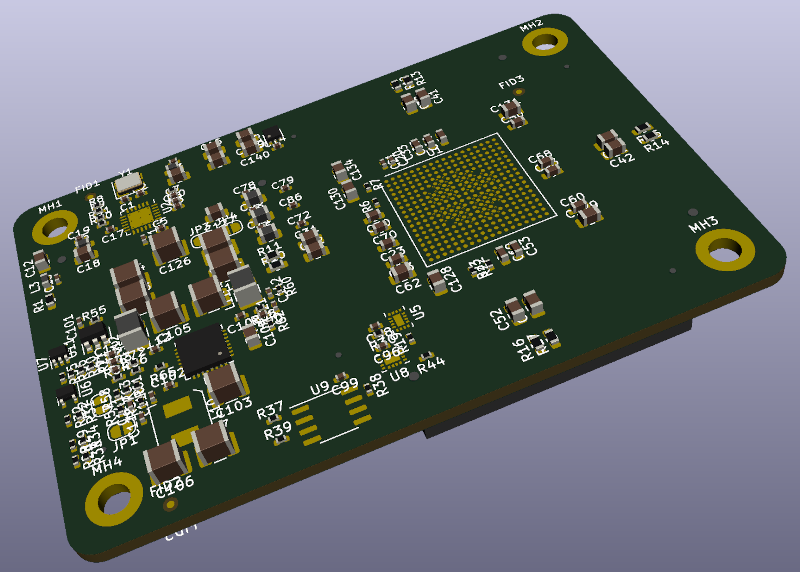
\includegraphics[height=3.5cm]{GMM-7550_preview_2020-10-01.png}
  \end{flushright}
  \vspace{-4cm}

  \begin{minipage}{9cm}
  \begin{itemize}
    \item an Evaluation Kit was not available back in mid-2020
    \item a module is smaller and reusable
    \item freedom for experiments\\(e.g. to interconnect several FPGAs)
    \item best way to get to know a new chip
    \item fun and easy exercise with KiCAD\\(at least it seemed so at the beginning)
  \end{itemize}
  \end{minipage}

\end{frame}

\begin{frame}
  \frametitle{Current Status}
  \begin{itemize}
    \item three boards designed and manufactured
    \item the boards are functional (from the very first versions and
    with just a few minor problems)
    \item schematic symbol and PCB footprint for GateMate FPGA are accepted
    into KiCAD v7 libraries
    \item control application is functional enought to debug, test,
    and configure the module
    \item several VHDL examples are running
    \item support for the module is (to be) added to the FuseSoC and LiteX
    (work in progress, nothing is upstreamed yet)
    \item \dots it took roughly 5 times longer than initially estimated
  \end{itemize}
\end{frame}

\section{Technical Details}

\subsection{Cologne Chip GateMate FPGA}

\begin{frame}
  \frametitle{GateMate FPGA Architecture (1/3)}
  \begin{itemize}
  \item novel CPE architecture (8-input LUT tree, two flip-flops or latches)
  \item low power consumption (GlobalFoundries 28~nm SLP (Super Low
  Power) process)
  \item 4 programmable PLL
  \item dual-ported block RAM
  \item 5 Gbps SerDes
  \item configuration via QSPI up to 100 MHz
  \item all pins configurable as single-ended (1.2 .. 2.5V) or LVDS
  \item all GPIO blocks support DDR
  \item 324-ball BGA, 15x15mm
  \end{itemize}
\end{frame}

\begin{frame}
  \frametitle{GateMate FPGA Architecture (2/3)}

  \begin{center}
    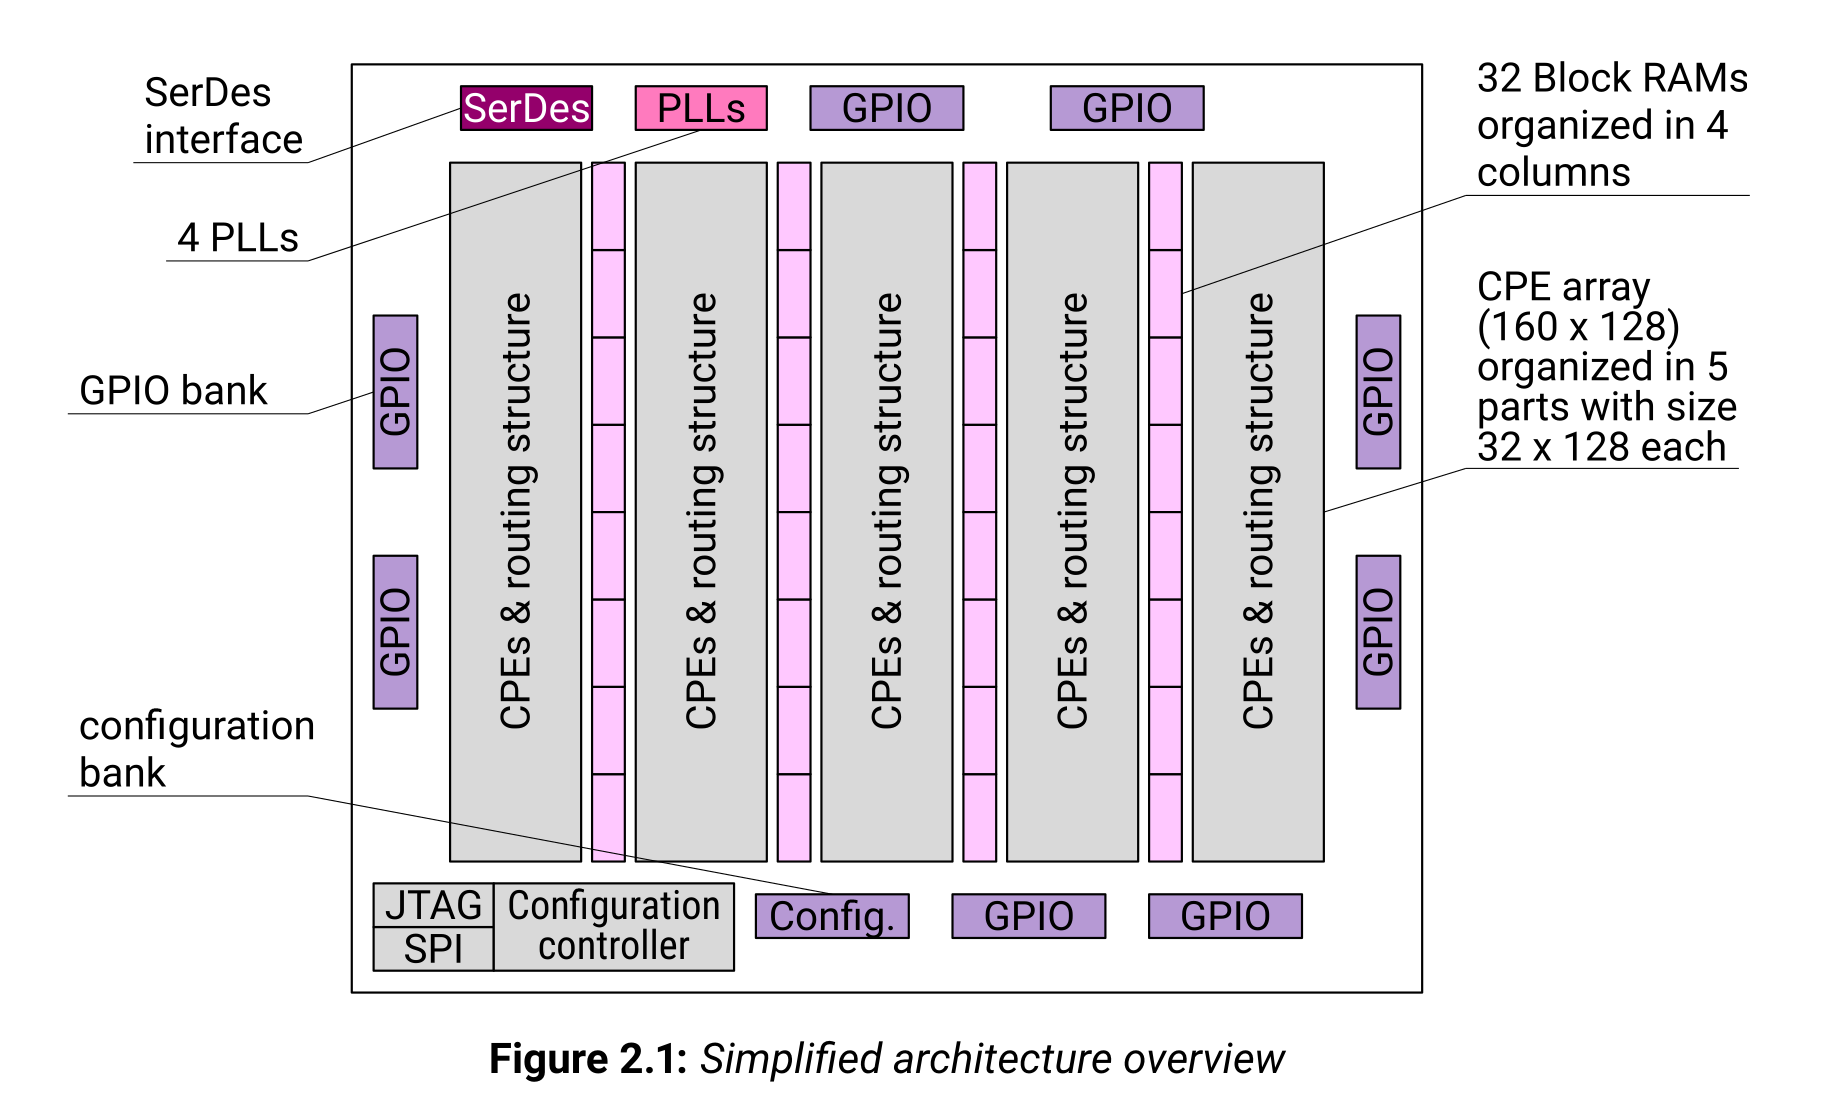
\includegraphics[height=6.5cm]{Figure_2.1.png}
  \end{center}
  \vspace{-2.5cm}
  \begin{flushright}
  \begin{minipage}{3.7cm}
  \footnotesize{{CologneChip~GateMate} FPGA Datasheet, DS1001, January 2023, page 21}
  \end{minipage}
  \end{flushright}
\end{frame}

\begin{frame}
  \frametitle{GateMate FPGA Architecture (3/3)}
  \vspace{-.5cm}
  \begin{center}
    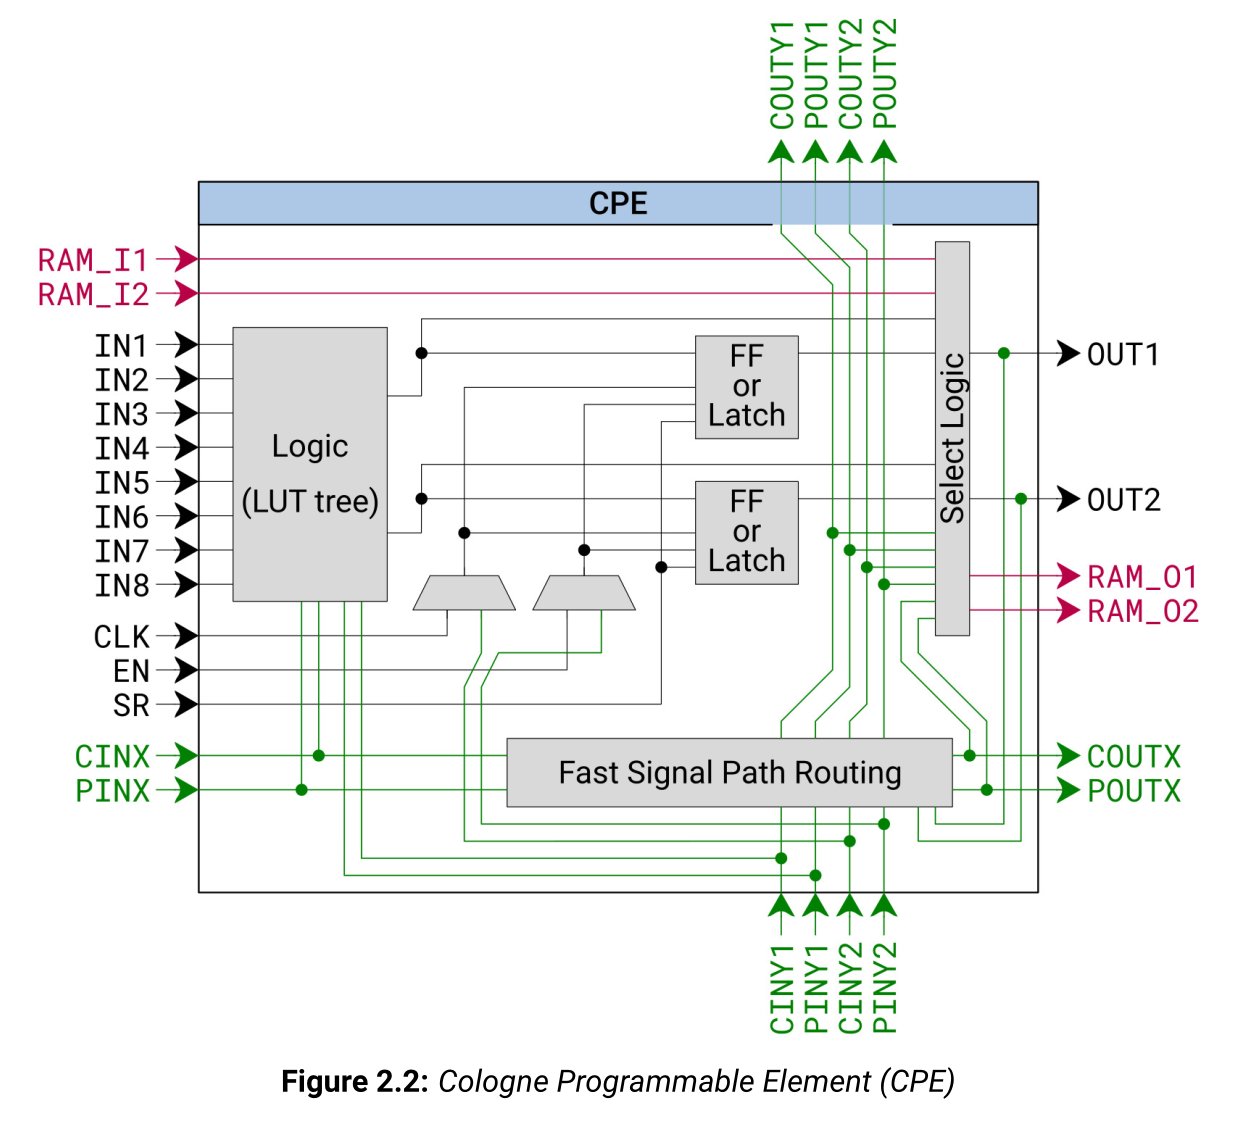
\includegraphics[height=7cm]{Figure_2.2.png}
  \end{center}
  \vspace{-2.5cm}
  \begin{flushright}
  \begin{minipage}{3.7cm}
  \footnotesize{{CologneChip~GateMate} FPGA Datasheet, DS1001, January 2023, page 22}
  \end{minipage}
  \end{flushright}
\end{frame}

\subsection{GMM-7550 Module}

\begin{frame}
  \frametitle{GMM-7550 Module -- Key Features}

  \begin{flushright}
    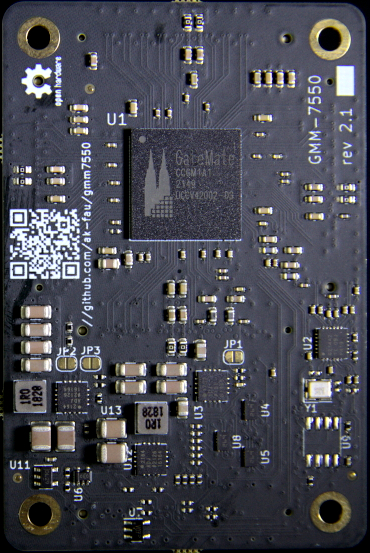
\includegraphics[height=5.5cm]{gmm7550.jpg}
  \end{flushright}
  \vspace{-5.5cm}

  \begin{minipage}{9cm}
  \begin{itemize}
  \item Cologne Chip GateMate FPGA CCGM1A1
  \item wide-range input power
  \item module control: discrete signals and I$^2$C
  \item 8 I/O banks available on 4 connectors\\with identical pinout
  \item 5 Gbps SerDes
  \item programmable clock
  \item all configuration modes are supported\\(Active and Passive SPI,
  and JTAG)
  \end{itemize}
  \end{minipage}
\end{frame}

\begin{frame}
  \frametitle{GMM-7550 Module -- Power}
  \begin{itemize}
  \item wide input range (2.9 .. 6.5V), may be powered directly from a
  3.3V baseboard, 5V USB, or single cell Li-Pol
  \item DC-DC are synchronized to the base clock and run in
  counter-phase\\(default 1.25~MHz, PLL programming option)
  \item 0.9/1.0/1.1V V$_{\text{core}}$ (build-time option)
  \item V$_{\text{io}}$ may be supplied directly on the module (2.5V, build-time
  option) or from\\a baseboard (individually for each I/O bank)
  \item ADP2164 step-down DC-DC, V$_{\text{io}}$ (2.5V) and V$_{\text{core}}$ are rated up to 4A
  \item separate LDO (ADP1753) for SerDes and SerDes PLL, 1.0/1.1V, 800mA
  \item input voltage monitor/reset generator on the module, an
  external reset input, and I$^2$C controllable reset
  \end{itemize}
\end{frame}

\begin{frame}
  \frametitle{GMM-7550 Module -- Clock}
  \begin{itemize}
  \item Texas Instruments CDCE6214 PLL with internal EEPROM
  \item 25~MHz crystal on the module
  \item LVDS reference clock input
  \item single-ended (LVCMOS 2.5V) and two differential output clocks
  \item default 100~MHz differential clock to the FPGA \texttt{SER\_CLK} input
  \item dedicated output for DC-DC synchronization
  \end{itemize}
\end{frame}

\begin{frame}
  \frametitle{GMM-7550 Module -- FPGA Configuration}
  \begin{itemize}
  \item JTAG (2.5V) available on the module connector
  \item Active Serial mode from SPI-NOR on the module or on a
  baseboard
  \item Passive Serial mode from a baseboard
  \item configuration mode and SPI connection configurable via I$^2$C
  \item SPI-NOR on the module is accessible from a baseboard
  \item \textbf{default mode:} Active Serial from SPI-NOR on the module
  \end{itemize}
\end{frame}

\subsection{Additional Modules}

\begin{frame}
  \frametitle{Raspberry-Pi 40-pin GPIO HAT Adapter}
  \begin{flushright}
    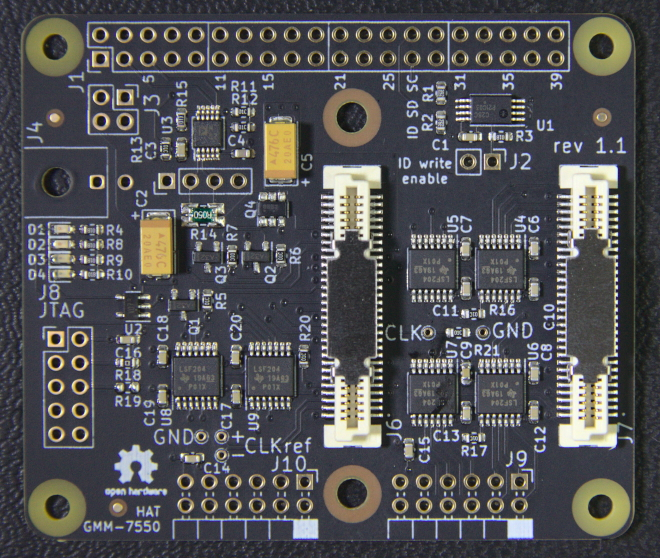
\includegraphics[angle=90, height=4.5cm]{hat-gmm7550.jpg}
  \end{flushright}
  \vspace{-5cm}

  \begin{minipage}{9cm}
  \begin{itemize}
  \item power for the module from R-Pi 5V or a separate power connector
  \item current and voltage monitoring (ADM1177)
  \item module control signals, I$^2$C, SPI, and UART
  \item 2x5 .1'' JTAG connector
  \item 2.5V/3.3V I/O level converters
  \item two 12-pin P-mod connectors for extension modules
  \item access to 3 I/O connectors
  \item 4x LEDs
  \item R-Pi HAT ID EEPROM
  \end{itemize}
  \end{minipage}
\end{frame}

\begin{frame}
  \frametitle{Memory Extension Module}
  \begin{flushright}
    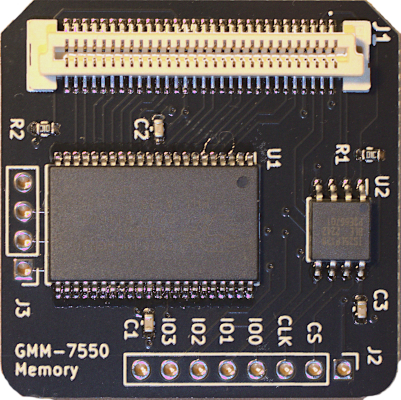
\includegraphics[height=3cm]{mem-module.jpg}
  \end{flushright}
  \vspace{-3cm}

  \begin{minipage}{9cm}
  \begin{itemize}
  \item SRAM 512K x8 (CY7C1049GN30-10ZSXI)
  \item QSPI-NOR 128Mb (16MiB, IS25LP128-JBLE)
  \vspace{.5cm}
  \item mechanical design validation
  \end{itemize}
  \end{minipage}
\end{frame}

\subsection{Software and RTL Code Examples}

\begin{frame}
  \frametitle{Control Application}
  \begin{itemize}
  \item Raspberry-Pi, VisoinFive
  \item ArchLinux ARM, \texttt{buildroot}
  \item CLI and web interface (Python panel)
  \item \dots live demo
  \end{itemize}
\end{frame}

\begin{frame}
  \frametitle{VHDL Examples}
  \begin{itemize}
  \item Yosys with ghdl-yosys-plugin, Cologne Chip \texttt{p\_r},
  GNU \texttt{make}
  \item GateMate primitives VHDL library
  \item blinking LED \textit{(with different clock inputs and PLL
  settings)}
  \item serial loopback
  \item SPI bridge to access SPI-NOR chips on the memory module\\
  from the baseboard SPI
  \item export examples as stand-alone projects
  \item \dots live demo
  \end{itemize}
\end{frame}

\begin{frame}
  \frametitle{Third-party Frameworks}
  \begin{itemize}
    \item FuseSoC
    \begin{itemize}
      \item blinky
      \item servant \textit{not working yet}
    \end{itemize}
    \item LiteX -- TODO
  \end{itemize}
\end{frame}

\section{What's next}

\begin{frame}
  \frametitle{Next steps -- for myself}

  To keep in mind in the future, that creating an open source hardware
  design takes the same effort and responsibilities as doing it ``for
  money'', just a bit more demanding,\\and no doubt is much more fun.

  \vspace{.5cm}

  \begin{itemize}
  \item test remaining things (SerDes, SRAM, ID EEPROM,
  operation at different V$_{\text{core}}$)
  \item stress test
  \item more examples, integration into frameworks
  \item RISC-V cores, software
  \item partial self-reconfiguration
  \item \dots
  \end{itemize}
\end{frame}

\begin{frame}
  \frametitle{Next steps -- for everybody}

  The greatest engineering reward and pleasure is to see the results
  of the efforts used by people, so, please:

  \vspace{.5cm}

  \begin{itemize}
  \item build modules, design baseboards and extension modules
  \item report problems
  \item create custom designs
  \item experiment
  \item share your results
  \end{itemize}

  \vspace{-3.5cm}
  \begin{flushright}
    \includesvg[height=3.5cm]{oshw-logo.svg}
  \end{flushright}

\end{frame}

\section{Contact info}
\begin{frame}

  \begin{minipage}{7cm}
    \vskip.5cm
    \huge{Thank you!}
    \vskip1cm
    \small{Anton Kuzmin}\\
    \small{\texttt{ak-fau+orconf@no-problem.cc}}\\
    \small{\texttt{https://github.com/ak-fau/}}
    \vskip.5cm
    \Huge{Questions?..}
  \end{minipage}

  \vspace{-5cm}
  \begin{flushright}
    \includegraphics[height=5cm]{github-vcard.png}\\
  \end{flushright}

\end{frame}


\end{document}
